\documentclass[11pt, a4paper ]{report}

\usepackage[utf8]{inputenc}
\usepackage[T1]{fontenc}
\usepackage[top=2.5cm, bottom=2.5cm, left=2.5cm, right=2.5cm]{geometry}
\usepackage[francais]{babel}
\usepackage{wrapfig}
\usepackage{graphicx}
\usepackage{makeidx}
\makeindex
%\usepackage{fontspec}
%\setmainfont{Arial}

\title{Mémoire Titre qui en jette grave}
\author{Julien Prugne 108287}
\date{Avril 2014 à Octobre 2014}

\begin{document}

	\maketitle
	\tableofcontents

	% TODO: à la toute fin
	\chapter*{Introduction} %3 pages

	% TODO: avant intro et conclusion
	% récolter assez d'info
	\chapter{présentation entreprise et mise en context : titre personalisé} % 25 pages

			%intro de partie
DOM Element Inc. est une startup Montrealaise. Elle à pour vocation de dévelloper et de promouvoire un produit. Ce produit c'est \emph{Happybox CMS}. Il s'agit d'une solution de création site web d'une seul page afin d'attirer l'attention sur un projet, un produit,...

Une startup\cite{theseStartup} est une jeune entreprise qui démarre. C'est une structure ayant pour but de déffricher un nouveau pan de l'economie. Il s'agit d'entreprise généralement incarné par leur(s) créateur(s) et foNdant son modéles économique sur l'innovation. 

L'entreprise en elle même n'est qu'une structure légale offrant une interface avec des stuctures ayant la capacité de financer l'essort du projet. En effet, les plan d'affaires de ces entreprises prévois généralement des pertes sur les premiers temps de son dévellopement voir pour l'intégralité de son existence. Cela peut sembler incohérent à premier abord mais un écosystéme c'est créer autour des startups. Riche particuliers\footnote{Bussiness Angel}, des groupe financier gérant un fond privé\footnote{venture capital}, concours entrepreunarial créer un flux entrant de capitaux dans cette économie. Ces derniers ont généralement pour objectif de rentabiliser leurs investissements lors de la vente ou de la capitalisation boursiére de la startup. Les montant en jeux sont considérable, les investissements ou les ventes de telle société ce chiffre généralement en dizaine,centaine de millier de dollars certain cas allant jusqu'à plusieurs milliards de dollars.

Les perspectives de ces marchés semble extrémement interessante mais il faut pondérer ces assertions par le taux d'échec impressionnant des start-up. En effet, une partie ne dépassera jamais le stade embryonaire, une grande partie arretera par manque de moyen financier empéchant de mener le projet à maturité, une petite portion sera acheter par de gros groupe\footnote{ skype, } et enfin une infime petite partie deviendront de large entreprise\footnote{exemple: facebook, twitter, Google,...} aprés capitalisation.
\begin{center}
\begin{tabular}{l*{1}{c}}
	Années  & Taux d'échec\\
	\hline
	1 & 25\% \\
	4 & 50\% \\
	7 & 63\% \\
	10 & 71\% \\
\end{tabular}\cite{statEchecStartup}
\end{center}

		\section{Présentation de l'entreprise: titre personnalisé} % 15 pages trouver un meilleur titre
			\subsection{Historique, de WebRight à Dom Element Inc}
		% présentation générale HappyboxCMS = intro plan d'affaire
		%	historique à étoffer
		\subsubsection{Happybox CMS, la plateforme web}
\paragraph{}
\emph{Happybox CMS}, a vu le jour en Octobre 2012, lorsque Guillaume Lagacé et Danny Coulombe, fondateurs de l'agence digitale \emph{WebRight\footnote{\url{http://webright.ca/fr}}} décident d'élaborer un moteur de création web alliant simplicité d'utilisation et téchnologie de pointe.
\paragraph{}
Pour arriver à leurs fins, ils enregistrent la société \emph{DOM Element Incorporated} le 23 Octobre 2012 auprés du registraire des entreprises du Quebec via la société \emph{Dufourd, Dion Avocats}. Les droits du produit Happybox CMS sont cédés à \emph{DOM Element Inc}, Danny et Guillaume se partagent alors la compagnie en deux parts égales, leur conférant un pouvoir décisionel commun et équivalent au sein de l'entreprise.
\paragraph{}
Durant les deux mois suivants, les efforts s'orientent sur le dévelopement du projet \emph{Happybox}. 
En décembre 2013, l'équipe rencontre Brendan Shera-Shriar et Brendan Tully-Walsh, co-fondateurs de l'agence de communication digitale \emph{The Brendans} qui deviendront, le 15 mai 2013 des actionnaires et membres éxecutifs de DOM Element Incorporated en échange de leur expertise en terme de communication et d'acquisition de clientèle.
\paragraph{}
Ce même mois de mai 2013, Happybox CMS, nom de produit approuvé plus tôt en fevrier, est sélectionné pour faire partie de la \emph{cohorte de la fondation Montreal Inc.} et recevra une bourse de \$12000. Bourse qui sera uilisée pour le financement du dévelopement et de la communication autour du produit.
\paragraph{}
En juin 2013, François Lacroix-Durant et moi-même intégrons les rangs de DOM Element Inc., respectivement en tant qu'intégrateur web et administrateur systémes.
\paragraph{}
À l'automne 2013, le service en ligne Happybox CMS ouvre ses portes pour une phase d'alpha privé comptant déjà une centaine d'utilisateurs. Principalement des dévelopeurs, des agences de Marketing Montréalaise ainsi que l'entreprise Maaco\footnote{Maaco est une des plus grande chaîne de peinture et de réparation de véhicules d'Amérique du nord.}.
\paragraph{}
Le 19 Novembre 2013, Happybox CMS se classe second au grand concours entrepreunarial \emph{Prix Montreal Inc}..
%%%%%% TODO: manquant décembre 2013 à maintenant %%%%%%%

%%%%%% FIN                                       %%%%%%%

			\subsection{Happybox CMS, une solution complète pour le web.}
		% présentation du produit avec screen et schéma technique (à traduire)

	% abstract
\paragraph{}
Happybox CMS est un logiciel en tant que service\index{SaaS!Happybox CMS}, c'est à dire qu'aucune installation n'est requise pour pouvoir l'utiliser. Il fonctionne sur un modèle client-serveur où le client est une page web dans votre navigateur communiquant avec un Service web, le serveur. Il faut le voir comme une feuille d'acétate qui se dépose sur un nom de domaine existant et permet instantanemment de créer un site web ou d'en éditer le contenu.

% Dom Element Inc c'est une stratup donc orienter sur 1 seul et unique produit

	% Présentation utilisateurs
	\paragraph{}
Happybox est avant toute chose un systéme de gestion de contenu\footnote{appellé aussi CMS, Content Management System}. Il s'agit d'un logiciel permettant la création et la mise à jour dynamique de site web. 
C'est un CMS spécialisé dans la création de site web à une seul et unique page, appellé aussi \emph{page d'aterrissage} ou \emph{landing page} en anglais. Ce type de site web est généralement réserver au opération de promotions qu'elles soient personelles\footnote{Pages personnelle, présentation d'un projet, CV en ligne, loufoquerie, ...} ou corporative\footnote{Bon de réduction, présentation d'un produit, évenements, ...}. Il a pour objectif d'interesser les internautes afin de les informer ou de les guider vers un autre service.

%%%%%% TODO: causer SEO %%%%%%

%%%%%%%%%%%%%%%%%%%%%%%%%%%%%% 

\paragraph{}
L'accés au service ce fait via une page Happybox présentant les différentes fonctionnalitées du logiciel. Cette page offre aussi un accés aux différents portails communautaires et à la création de compte. Ce site est une vitrine des possibilité offerte par le CMS. C'est le point d'accroche de la communication autour du produit.

%% SCREENSHOT ACCEUIL HAPPYBOX %%

\begin{center}
		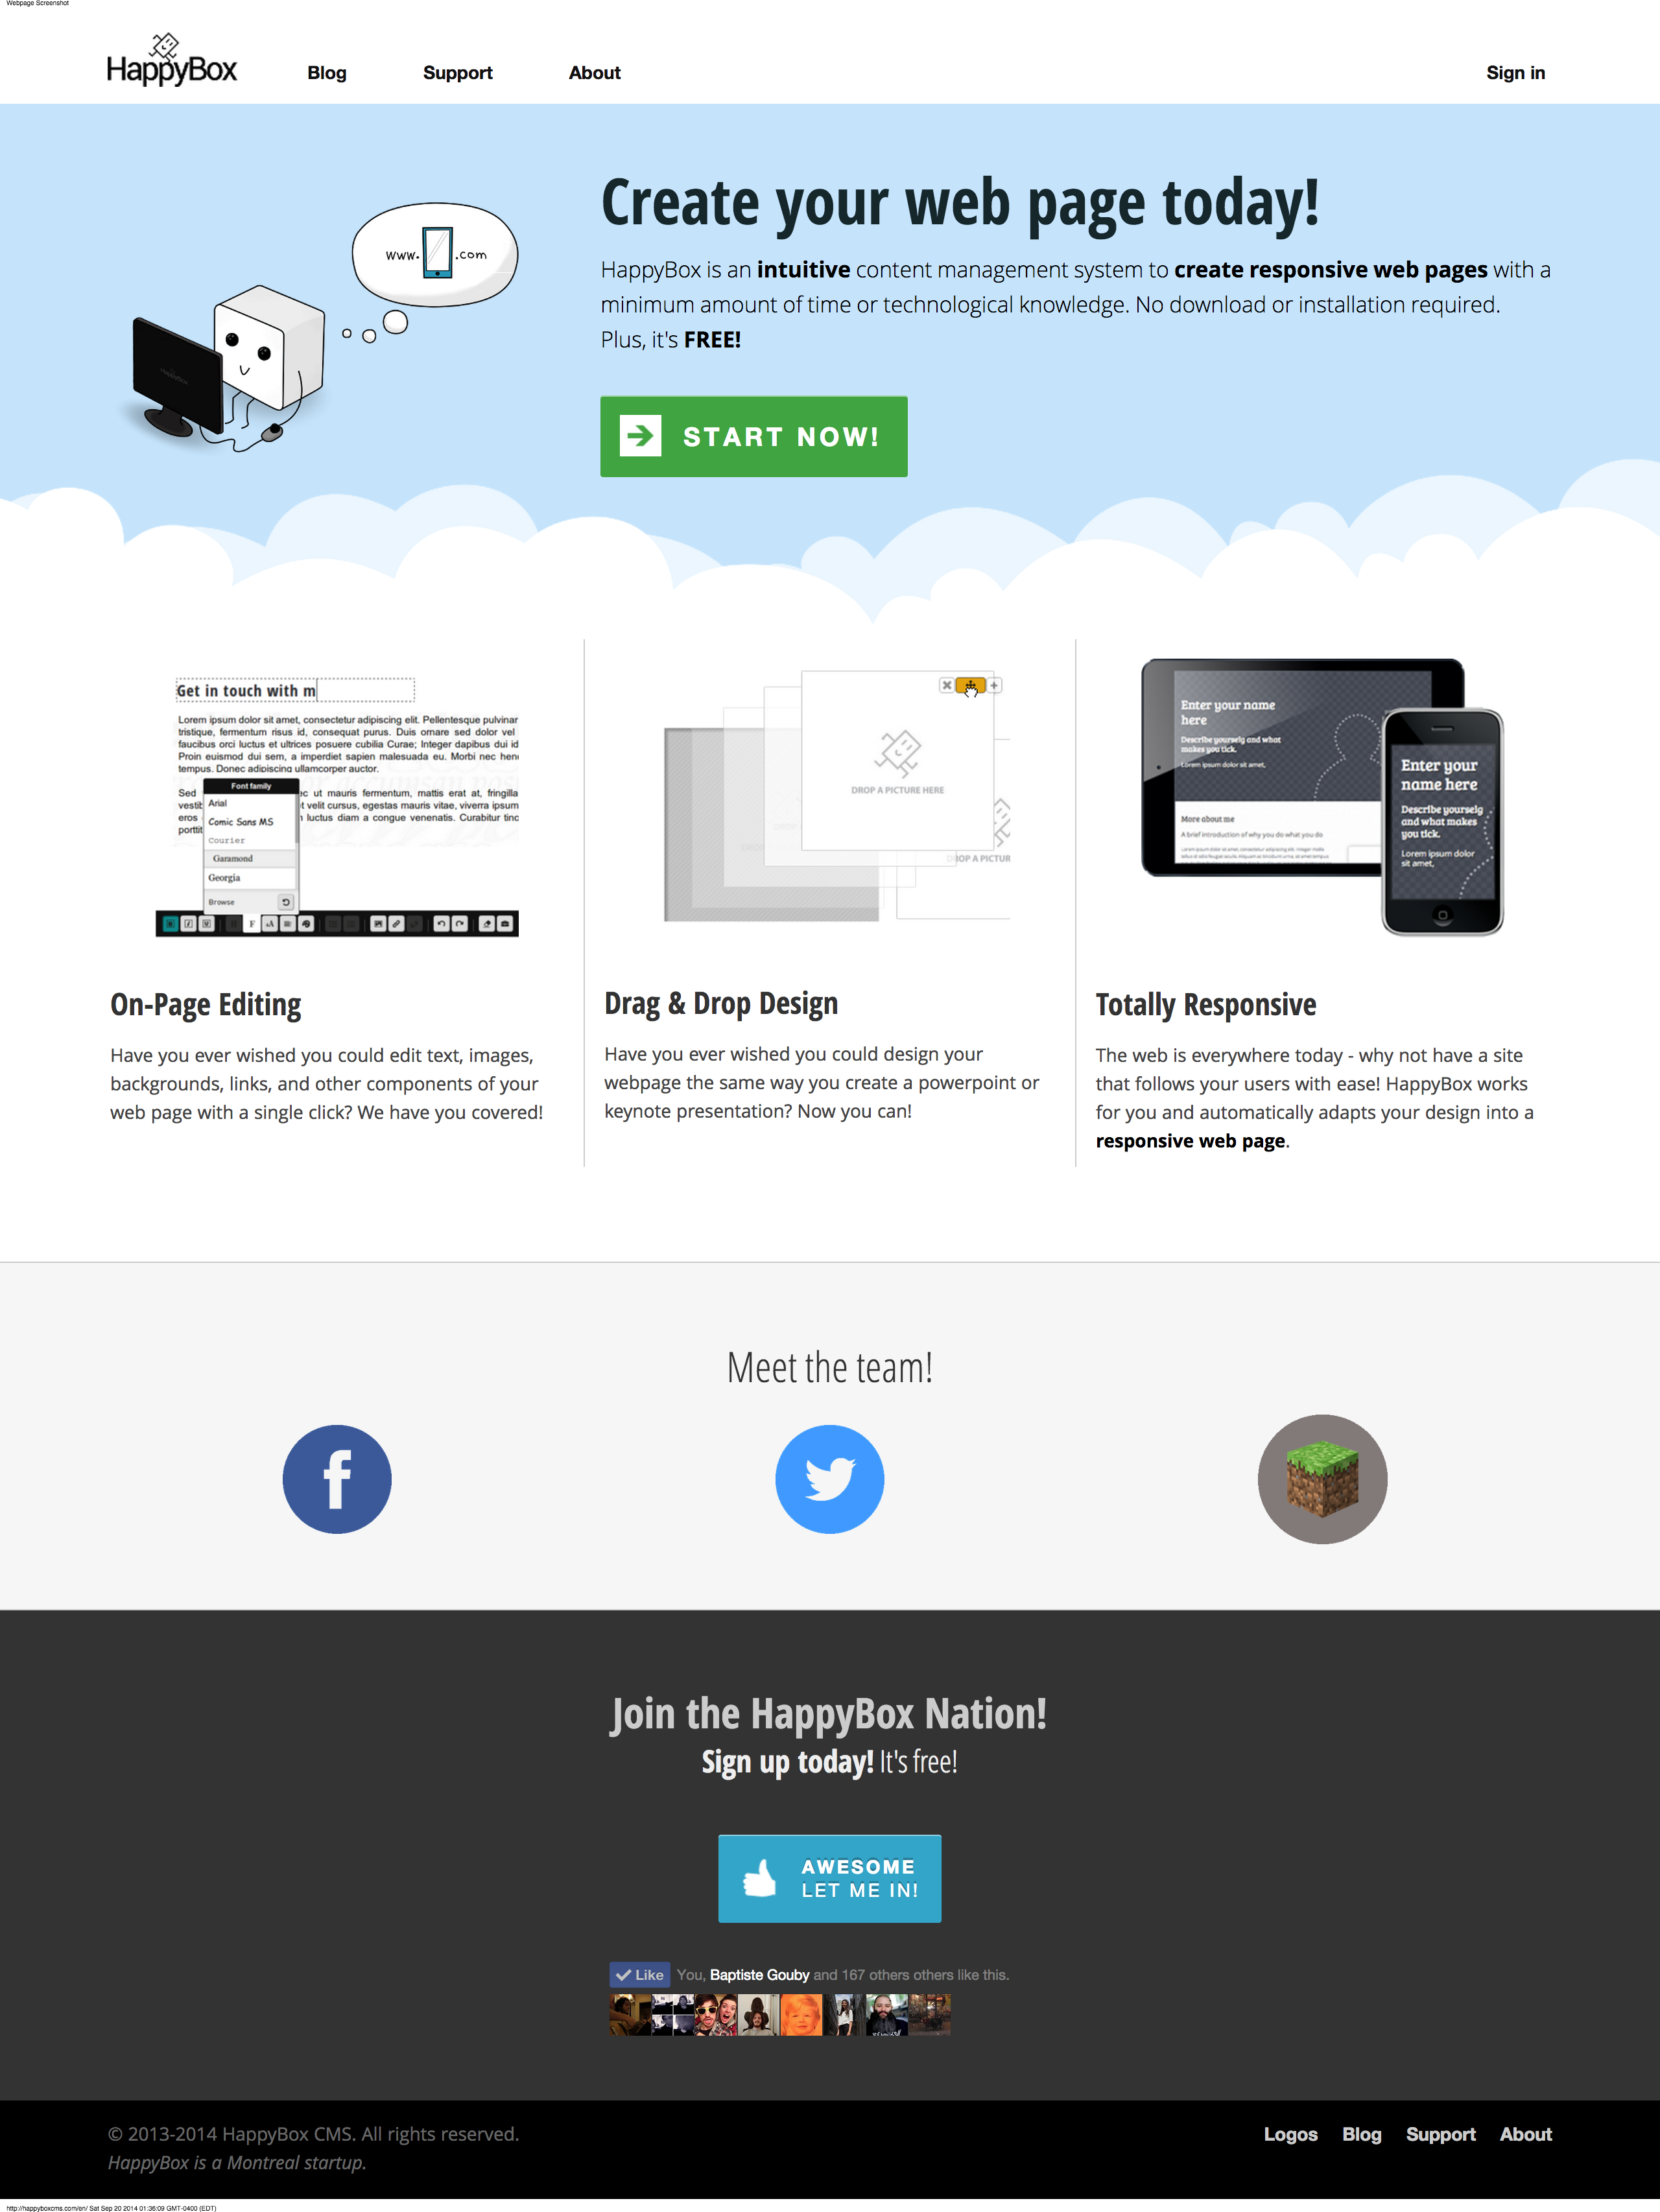
\includegraphics[width=\textwidth]{images/HBscreen/fullLanding.png}
		\caption{\url{http://happyboxcms.com} - Page d'aterrissage}
\end{center}

\paragraph{}
En effet Happybox CMS propose un éditeur de page intuitif, permettant en quelques cliques de définir un gabarit ou template de page. Le moteur ce base sur un systéme de grille, en effet les pages sont définies comme étant un ensemble de ligne ou section superposé les unes aux autres. Ces lignes peuvent être visibles ou non afin de créer des séparateurs sur la page\footnote{Section invisible laissant apparaitre le fond de la page.}. Dans ces sections, il est possible de définir des colonnes d'une largeur définis lors de la création du gabarit. Ces colonnes sont des conteneurs qui nous permettrons de stocker le contenue de la page par l'intermédiaire de \emph{widget\footnote{Élément textuel, titre, images, formulaire de contacts, liens, ...}}.

Chaque gabarit est complétement \emph{responsive\index{responsive!moteur de gabarit}}, c'est à dire qu'il s'adapte automatiquement à la résolution du navigateur client afin de garantir la meilleur expérience d'utilisation quelque que soit la plateforme utiliser pour consulter un site créer avec HappyboxCMS. La fonction de prévisualisation ainsi que les boutons en bas de l'éditeur permettent de tester son site pour chaque type d'appareil.


%% SCREENSHOT EDITEUR DE GABARIT%%
\begin{center}
	
		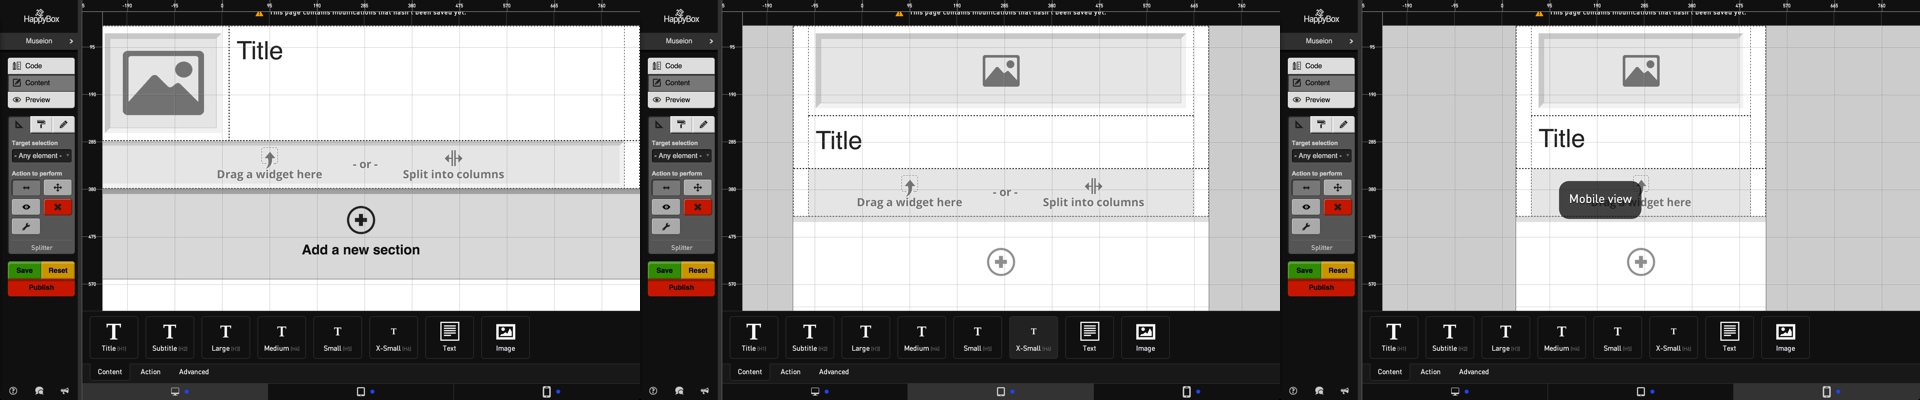
\includegraphics[width=\textwidth]{images/HBscreen/editeurGabarit.png}
		\caption{Editeur de Gabarit: vue ordinateur, vue tablette, vue mobile}
	
\end{center}

\paragraph{} % contenue, style, SEO
Une fois qu'une page est structuré il faut lui ajouter un style. Pour cela, un éditeur de style complet permettant de gérer la majorité des propriétées css via une interface simple d'utilisation permettant aux non-developeur d'affiner leur design avec un niveau de détails inégalé. Pour les utilisateurs confortable avec l'édition d'un fichier css, il possible d'écrire directement du code css dans l'éditeur. 
Le contenue de la page, textes, images, sont éditable directement sur la page avec un rendu en temps réel. Ce que vous voyez c'est ce qui sera affiché.
Happybox garde en mémoire que la fonction premiére d'une page d'aterrissage est avant tout un outils de référencement vous permettant d'offir une meilleur visibilité à un produit ou un service pour le web. Un assistant de SEO est disponible dans l'éditeur proposant d'améliorer votre page en temps réel afin que les moteurs de recherche index au mieux la page.
%% screen contenue style CEO
\begin{center}
	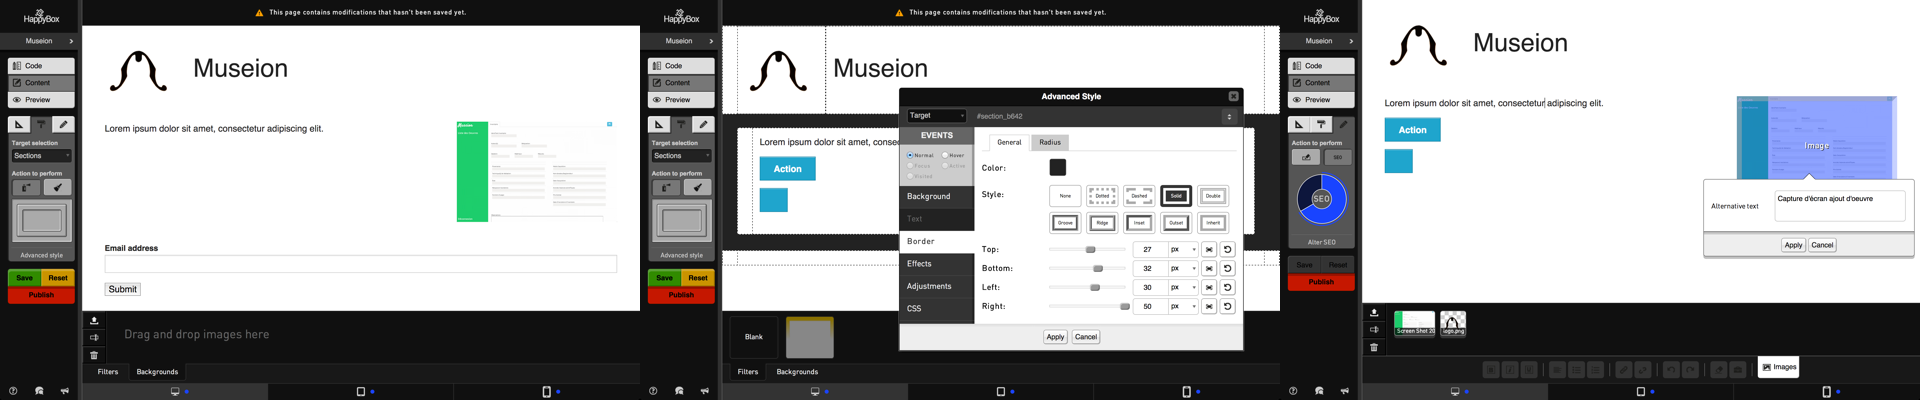
\includegraphics[width=\textwidth]{images/HBscreen/contenueStyleSeo.png}
	\caption{Editeur de contenue, editeur de style, editeur de SEO}
\end{center}

\paragraph{} % editeur de code + versionning
Happybox ciblant prioritairement les developeurs web, c'est pourquoi un éditeur de code permettant d'éditer l'intégralité des source de la page et d'ajouter des modules php ou javascript afin d'étendre encore les possibilités de la plateforme. Ce qui n'est pas déjà dévelopé par l'équipe pourra être dévellopé et tester avec un rendue en temps réel. 
%% Screenshot editeur de source
\begin{center}
	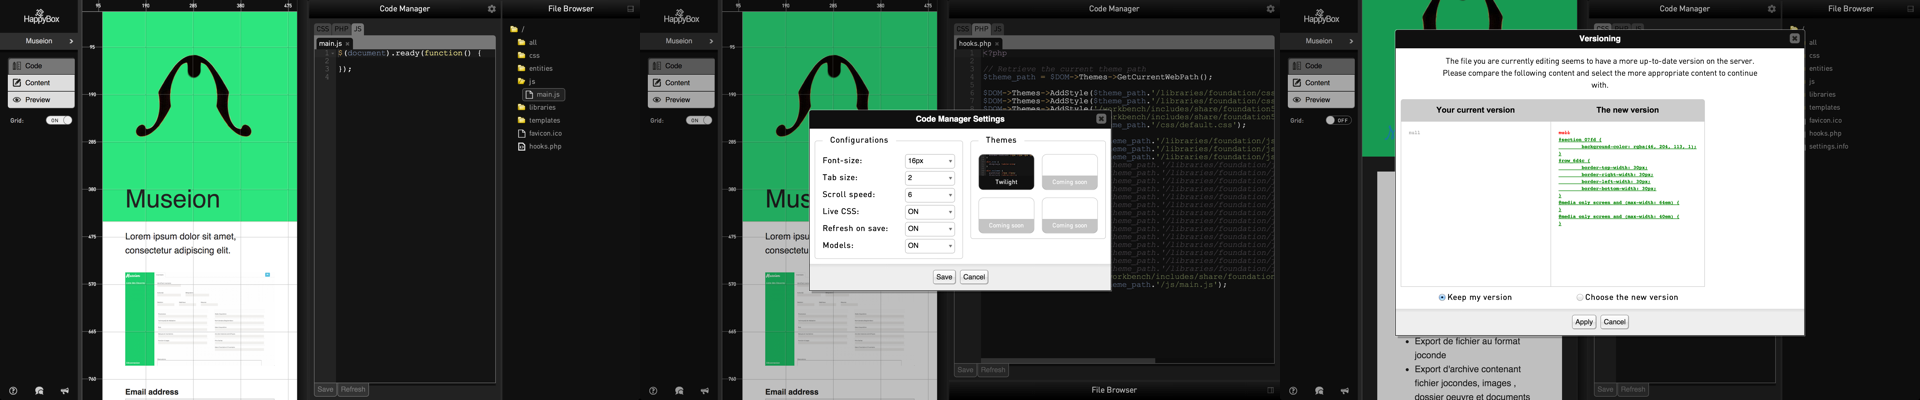
\includegraphics[width=\textwidth]{images/HBscreen/codeManager.png}
	\caption{Editeur de code: fichier php, configuration, gestion des versions}
\end{center}

% séparation fond et formes
\paragraph{}

\begin{center}
	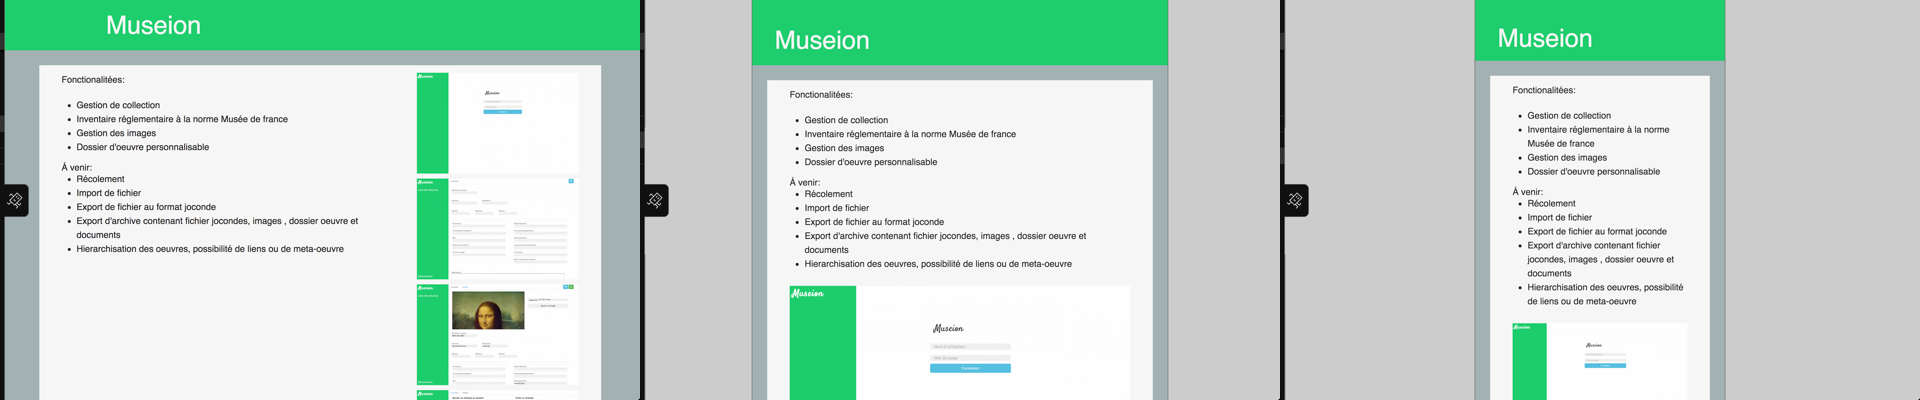
\includegraphics[width=\textwidth]{images/HBscreen/preview.png}
	\caption{Prévisualisation de la pages version ordinateur, tablette et mobile}
\end{center}

% présentation des outils de gestions
\paragraph{}
De plus chaque client ce vois allouer un espaces dédié sur nos serveurs. Il reste ainsi le seul et l'unqiue propriétaire de ses données. Happybox est donc aussi un hébergeur de données. 
Des services d'analyse de traffique, de gestion de consommation, de nom de domaines et gestion de projet sont aussi mise à dospistion des utilisateurs.

\begin{center}
	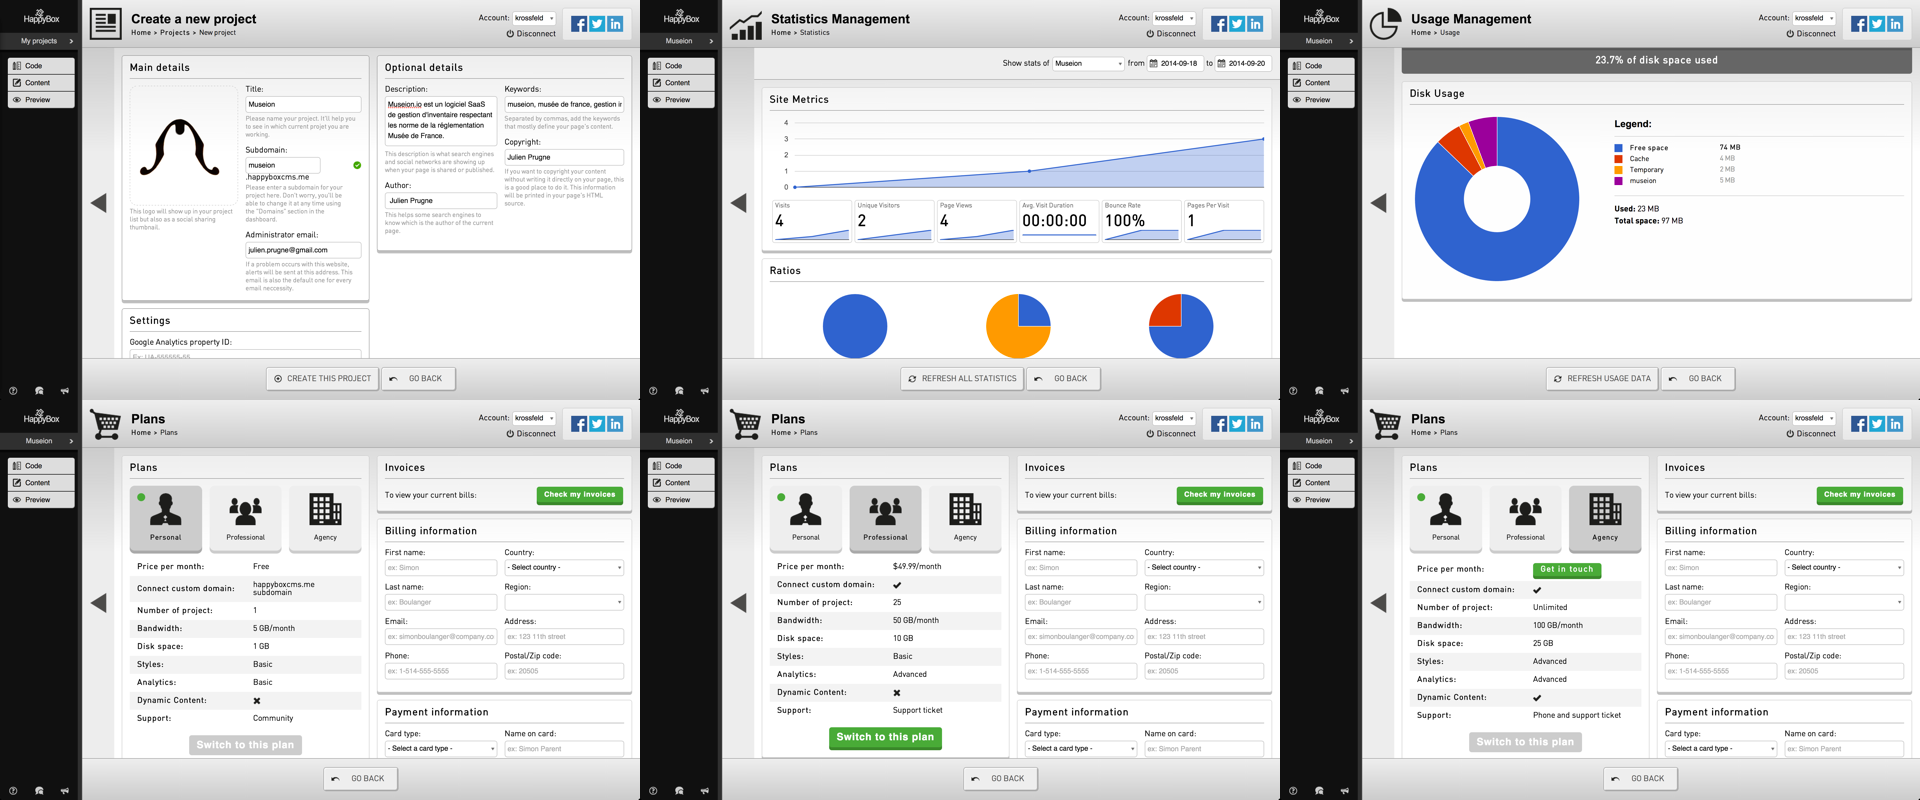
\includegraphics[width=\textwidth]{images/HBscreen/dash.png}
	\caption{Differentes options du panneau d'administration et différents forfait proposé}
\end{center}



% analyse que c'est un bon CMS
Il répond donc à un certain nombre de fonctionnalitées communes à l'ensemble des systémes de gestion de contenue et recherché par les utilisateurs de CMS\cite{enqueteCMSSmile}.

\begin{itemize}
	\item Structuration du contenue 

		\begin{itemize}
			\item Durant la création de votre page Happybox 

			\item Contenus structuré 

			\item Organisation des contenus 

		\end{itemize}

	\item Ergonomie des outils de gestion 

		\begin{itemize}
			\item Qualité de l'interface de gestion 

			\item Dépot de contenu Wysiwig 

		\end{itemize}

	\item Experience utilisateurs en front-office 
		\begin{itemize}
			\item Souplesse des gabarits et mise en page 

			\item Accessibilité 

			\item Référencement 

			\item Personnalisation 

			\item Référencement 
			\item Receuil d'information/formulaire 

		\end{itemize}

	\item Processus de publication 
		\begin{itemize}
			\item Gestion de la version du contenue 

			\item Cycle de vie du contenue 

			\item Travail collaboratif 

		\end{itemize}

	\item Intégration avec les réseaux sociaux 

	\item Qualité de l'architecture technique 
		\begin{itemize}
			\item Documentation

			\item Plugins et extensibilité

			\item Performances 

		\end{itemize}

\end{itemize}




			\subsection{Plan d'affaire}
		% plan d'affaire
			% chiffre
			% stratégie d'accés au marché 

		% annex le plan d'affaire d'happybox
			% présenter
		% mon analyse 
		%l'état actuel d'happybox

		%ma proposition de futur
			% conteneur opensource

			\subsection{Management orienté produit}
		% Fonctionnement de l'entreprise


		\section{Mise en context} % 10 pages


			\subsubsection{Entrepreunariat à Montreal}
				% communauté tech
				% communauté entrepreunarial et startup
				% entrepreunariat sauvage

			\subsubsection{Concurence}
				% wix


	\chapter{Problématique} % 28 pages
		\section{problématique} % 5 pages



Il est de plus en plus courant de recourir au service de cloud\footnote{appelé aussi informatique en nuage} public afin de gagner en perfomance, en disponibilité, de simplifier les taches d'administration en faisant abstraction de la couche matérielle.
Malgrès leurs apparences attirantes les plateformes dites IaaS, Infrastructure as a Service\footnote{Infrastructure comme un Service}, engendre un lot de coût plus ou moins caché et de nouveaux défis dans la gestion des systèmes d'information. Il semble donc nécessaire de mettre en place une politique de gouvernance afin de réellement exploiter le potentiel de telles infrastructures.
Mais quels sont concrétement les éléments constitutifs d'une telle démarche.

			%Explication et developement de la problématique
			\subsection*{}
				%terminologie
				%\subsubsection*{}

Avant d'aborder le vif du sujet il me semble nécessaire d'expliciter un certain nombre de termes et concepts qui sont utilisés dans la problématique et s'avèrent fondamentals à la compréhension de ce document.
					%cloud
					%\paragraph{}
						%definition Cloud computing en géneral

Le cloud computing\cite{cloudDef}\index{Cloud computing!Définition} est une pratique visant à dématérialiser les infrastructures des services d'information. Elle entraine un changement fondamental dans le paradigme d'accès aux ressources informatiques. En effet, les machines hôtes ne sont plus accessibles physiquement mais virtualisées à l'aide d'un hyperviseur\index{Hyperviseurs}.

Les hyperviseurs sont des plateformes de virtualisation permettant d'éxécuter plusieurs systémes d'exploitation dit invités\index{systéme invité} sur une même machine dite hôte\index{systéme hôte} ou une ferme de calcul\footnote{Appelé également grappe de serveurs ou encore cluster. Il s'agit d'un ensemble d'ordinateurs reliés les uns aux autres, mettant leurs ressources en commun, créant ainsi une sorte de \emph{super ordinateur}. }.

Cela crée ainsi une abstraction entre la gestion physique du matériel et l'exploitation des ressources informatiques. Ainsi, la mise en place d'un serveur ne se fera plus en achetant et en installant un nouvel hôte dans son centre de données, mais via la réservation et la création de machines virtuelles.

Un hôte physique hébergera donc un ou plusieurs systèmes d'exploitation et l'hyperviseur se chargera d'allouer ou non les ressources\footnote{unité de calcul, mémoire, stockage, accès réseaux, ...}  physiques nécessaires via des interfaces virtuelles accessibles depuis la machine virtuelle comme si ces derniers étaient physiques. Le système invité ce comportera comme si il possédait son propre matériel.

Les nuages peuvent être classés dans deux catégories: les cloud privés et les cloud publiques.

						% définition cloud privé

Les cloud privés\index{cloud privé|nuage privé! définition} sont des infrastructures physiques\footnote{serveur isolé ou en grappe} loués ou hébergés dans un centre de données et uniquement utilisés par le locataire ou propriétaire. Ils sont physiquement accessibles par les administrateurs qui seront responsables de leur bon fonctionnement. Si les ressources fournies par le nuage privé viennent à manquer, il sera du ressort des exploitants\footnote{propriétaire ou locataire des infrastructures} d'acheter, de configurer et d'installer un nouvel hôte dans la ferme de calcul afin d'augmenter les ressources allouables aux systémes invités. Á puissance égale ces infrastructures semblent moins dispendieuses que les cloud publiques mais les moyens humains nécessaires à la mise en place et la maintenance de telles solutions sont conséquents.

						% définition cloud public
Les seconds, dis nuage public\index{cloud public|nuage public! définition}, sont des infrastructures accessibles généralement via des applications web et/ou des interfaces de programmation\footnote{API: Application Programming Interface}. Les ressources sont accessibles en libre service et à la demande. Le prestataire facturera à l'utilisation\footnote{Exemple: volume de données hébergées, mémoire utilisée par une application, bande passante, ...} ou de manière forfaitaire\footnote{Location annuelle d'une instance, réservation d'un espace de stockage dédié, ...}.

					%\paragraph{IaaS/PaaS/SaaS} transition TODO:definir serrvice web
					%utiliser pizza as a service comme exemple
				% résumé
Les clouds publiques sont generalement composés de trois types de services\index{service|service web!définition}\footnote{Un service web\cite{webServicesDef} peut être défini comme étant une interface logicielle permettant un accès standardisé à un ensemble de ressources hétérogènes via internet ou un réseau intranet.}:
\begin{description}

	\item[IaaS\index{IaaS|Infrastructure as a Service}, Infrastructure as a Service, Infrastructure comme un Service] Amazon Web Services, Google Compute Engine, Digital Ocean

	\item[PaaS, Plateform as a Service, Plateforme comme un Service] Heroku, Google App Engine, dotCloud, Amazon Opswork

	\item[SaaS, Software as a Service, Logiciel comme un Service]
	Happybox CMS, Gmail, Jira, Museion

\end{description}

Pour bien expliquer ces différents concepts, nous nous réfererons à l'excellente analogie \emph{Pizza comme un Service}\cite{PizzaasaService}. Cette dernière nous explique que les habitudes d'utilisation de plateforme en ligne sont comparables aux habitudes de consommation de pizza.

En effet, un cloud privé\index{Cloud privé!Définition par la pizza} où vous vous chargeriez d'équiper les locaux en éléctricité, en ventilation, de gérer la sécurité physique et logicielle et installer les serveurs dans votre centre de données serait comparable à faire votre pâte à pizza, garnir votre pizza, la cuire, installer votre table à manger, servir les boissons et votre pizza. Cette solution vous offre le plus de fléxibilité dans les choix que vous pouvez faire mais peut devenir très contraignante car tout est de votre responsabilité. 

Les solutions IAAS\index{IaaS!Définition par la pizza}, sont comparables au fait d'acheter une pizza crue ou congelée et de la cuire chez vous. En d'autres termes vos considérations s'orienteront sur le choix et l'installation des sytémes d'exploitations, la création de réseaux virtuels, la configuration de gestionnaire de charge\footnote{load-balancer}... Ces services vous offrent un centre de données complet sans les inconvénients du matériel. 

Les solutions PaaS\index{Paas!Définition par la pizza} correspondent au service de livraisons de pizza. Il ne reste à votre charge que la table et les boissons. D'un point de vue informatique, vous géreriez la création de votre application puis la déploierez chez votre fournisseur. La gestion du systéme d'exploitation n'est plus de votre ressort vous laissant la responsabilité de votre logiciel.

Finalement les solutions SaaS\index{SaaS!Définition par la pizza} sont le pendant logiciel des pizzerias. Il vous suffit de payer, ou de laisser la plateforme collecter vos informations personelles en guise de paiement, pour accéder aux services et rien n'est de votre ressort à part votre utilisation. Il s'agit d'une évolution de la livraison et de la consommation logicielle.

Le schéma ci dessous illustre ces explications:

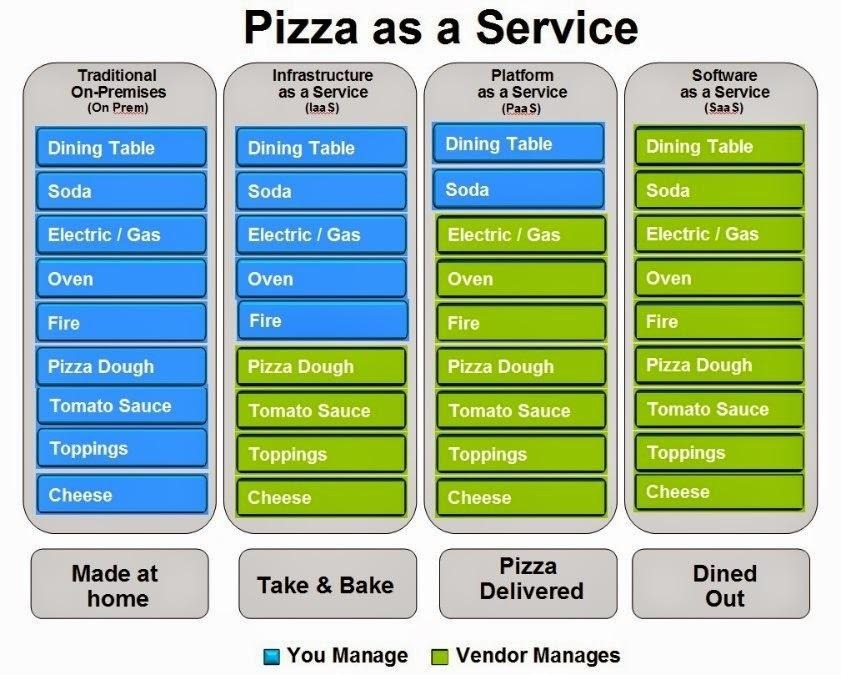
\includegraphics[scale=0.5]{images/PizzaasaService.jpg}

				%\subsection*{approche envisagé}

					%\paragraph{cout}
					%\paragraph{consitence de la conf}
					%\paragraph{sécurité et privacité}
La frontière entre ces différents types d'infrastructure est parfois mince voire inexistante. Par expemle, la plateforme web permettant de gérer ses infrastructures virtuelles chez n'importe quel fournisseur d'infrastructure comme un service\footnote{IaaS} n'est autre qu'un logiciel comme un service\footnote{SaaS}. De plus, les plateformes IaaS fournissent généralement une solution de plateforme comme une service\footnote{PaaS}. Google app Engine est une plateforme PaaS fournis par google et inclus dans l'offre Google Cloud, de la même façon Amazon Web Service propose Opswork. 

De fait, ces concepts restent trés théoriques et leurs implémentations ne sont jamais une vision absolue du concept. Il est donc important de bien comprendre ces services afin de définir le potentiel de chaque plateforme d'hébergement et d'en exploiter au maximum les fonctionnalitées. 
Pour cela, nous utiliserons sept d'indicateurs permettant, selon mon expérience, de comparer la pertinence des différentes solutions présente sur le marché. 

\begin{description}

	\item[Sécurité] 
		Controller l'accès aux ressources et aux données. Pouvoir garantir leur confidentialité.

	\item[Souveraineté]  
		Posséder totalement ou partiellement ses ressources et données.

	\item[Adaptabilité]
		Changer, ce transformer, s'adapter aux besoins des utilisateurs.

	\item[Consistence]
		Garantir la configuration, les mises à jours.

	\item[Cout]
		Le nerf de la guerre qu'il faut savoir gérer pour ne pas ce retrouver sans éléctricité pour ses serveurs.

	\item[Compétence nécessaire]
		Besoin en formation ou en personnel qualifié.

\end{description}

Ces indicateurs, devrait à eux seuls permettre de définir notre politique de gouvernances. Ils sont, en quelques, sorte les indicateurs vitaux d'un systéme informatique. 

		% Méthodes habituellement utilisé pour une situation présentant des similitude
		\section{méthodes habituelles} % 5 pages
			\subsubsection{location chez OVH ou autre}
			\subsubsection{création d'un datacenter}
			\subsubsection{Déploiement manuel ou scripté}

		% Exposé des décisions prise et des interventions menée par le stagiare pour résoudre le problème
		\section{truc fait}	 % 15 pages

			\subsubsection{Déploiement happybox CMS}
				% montrer que ça demande beaucoup de temps et d'efforts
				% peu de moyen et peu de monde
			\subsubsection{AWS}
				% analyse des coups, explication IAAS
				% présentation argumenté de AWS/GCE

			\subsubsection{Opswork}
				% gestion configuration, automatisation déploiement, productivité

			\subsubsection{Open source: Gitlab, Open Web Analytics}
				% impact du logiciel libre sur le travail
				% Ouverture sur le possible future libre de Happybox CMS

		% Démonstration d’une originalité dans l’élaboration et la mise en œuvre de la solution
		\section{Demonstration que c'est trop plus la bonne décision} % 5 page
				% gain productivité
				% gain cout
				% gain maintenabilité
				% gain scalabilité
				 % gain sécurité

		% Analyse de l’approche choisie
		\section{Analyse masturbatoire de l'action} % 3 pages
				% c'est le monet de ce la péter

		% Réflexion sur le stage et le mémoire
		\section{Autoévaluation}

	\chapter*{Conculsion} % 2 pages

	\chapter*{Remerciements}

	\appendix
	\section{Exemple de pages Happybox}
	%bibliographie
	\printindex

	\bibliographystyle{amsplain}
	\bibliography{bibli}

\end{document}
